\documentclass[10pt,letterpaper,subeqn]{beamer}
\setbeamertemplate{navigation symbols}{}
\usefonttheme{serif}
\usecolortheme{seahorse}



\usepackage[english]{babel}
\selectlanguage{english}
\usepackage{bm}
\usepackage{booktabs}
\usepackage{color}
\usepackage[update,prepend]{epstopdf}
\usepackage{framed}
\usepackage{fleqn}
\usepackage{graphics}
\usepackage{hyperref}
\usepackage[utf8]{inputenc}
\usepackage{setspace}
\usepackage{textcomp}
\usepackage{wrapfig}
\usepackage{multirow}
\usepackage{caption}
\usepackage{subcaption}
\usepackage{subfloat}
\setbeamertemplate{caption}[numbered]
\usepackage{wrapfig}
\usepackage{tikz}

\definecolor{cadmiumgreen}{rgb}{0.0, 0.42, 0.24}
\usetikzlibrary{trees}
\usetikzlibrary{decorations.markings}


%================================================================================
%== TITLE, NAMES, DATE
%================================================================================
\title{The Value of Season of Birth and Fertility Timing}

\author{Damian Clarke\inst{\dag} 
   \and Sonia Oreffice\inst{\ddag} 
   \and Climent Quintana-Domeque\inst{*}}

\institute{\inst{\dag}  University of Oxford
      \and \inst{\ddag} University of Surrey and IZA 
      \and \inst{*}     University of Oxford and IZA}

\date{June 2015}
%********************************************************************************
\begin{document}


\begin{frame}
\titlepage
\end{frame}
%********************************************************************************

\begin{frame}[label=Motivation]
\frametitle{Motivation}

\begin{itemize}
\item Season of birth relevant for birth quality and long-term outcomes:
      \begin{itemize}
        \item child health, educational attainment, labor market
        \item Buckles and Hungerman (2013)
        \item Crawford et al.\ (2014)
        \item Currie and Schwandt (2013)
      \end{itemize}
\item Although no consensus yet on the main driving force: 
      \begin{itemize}
        \item selection (of mothers), school entry rules, weather in last term (winter)
      \end{itemize}
\item The \emph{effects} of the season of birth are clear: there are ``good'' 
and ``bad'' seasons
\end{itemize}
\end{frame}

%-------------------------------------------------------------------------------
\begin{frame}[label=Motivation2]
\frametitle{Motivation}
Winter months are bad: quarters 1 and 4, Spring and Summer are good (quarters 2 
and 3), at least in the US \\ \vspace{4mm}
However,
\begin{itemize}
  \item No analysis of the \emph{determinants} of the season of birth of a child
  \item[$\rightarrow$] We consider the choice of season of birth
\end{itemize}
\vspace{6mm}
Fertility planning and season of first birth: 
\begin{itemize}
  \item When to have the first child and in which season?
  \item Focus on SOB decision, take age of mother as given
\end{itemize}
\end{frame}


%-------------------------------------------------------------------------------
\begin{frame}[label=map]
\frametitle{What do we do?}

\begin{enumerate}
\item Correlates of season of birth with mothers' attributes
\item Correlates of season of birth with child quality
\item Use gestation weeks to further disentangle the expected from the realized good and bad seasons
\item Age is the most important determinant of SOB
\item Why? Preferences and/or biological constraints?
\item Estimate value of SOB in terms of birth quality 
\item Value of SOB and postponing fertility, trade-off:
      \begin{itemize}
       \item Postpone: earnings increase but less good season
       \item Not postpone: earnings decrease but good season
      \end{itemize}
\end{enumerate}
\end{frame}

%-------------------------------------------------------------------------------


\begin{frame}[label=how]
\frametitle{How do we do it?}

\begin{itemize}
\item US and Spain: birth certificates
\item Reduced-form estimates of season of birth, also by smoking during pregnancy and ART use
\item Reduced-form estimates of birth quality, season of birth, also by mother's attributes
\item Bare-bones model:
      \begin{itemize}
        \item two types of women, young and old
        \item SOB is choice variable
      \end{itemize}
\item Structural model: work in progress, to assess the value of SOB, importance of 
biological and economic constraints
      \begin{itemize}
        \item Two endogenous variables: age and SOB 
      \end{itemize}
\end{itemize}
\end{frame}
%-------------------------------------------------------------------------------

\begin{frame}[label=datades]
\frametitle{Data Description}
\begin{itemize}
\item US National Vital Statistics System: all birth certificates
\item Detailed information on ``birth quality'' and mothers' characteristics
\item We focus on:
      \begin{itemize}
        \item White and non-Hispanic women who had their first-born child
        \item Singletons (we also look at twins)
        \item Mothers aged 25-45
        \item 2005-2013
      \end{itemize}
\end{itemize}
\end{frame}



\begin{frame}[label=sum]
\input{./tables/sumStatsnvss.tex}
\end{frame}

\begin{frame}[label=BQs]
\input{./tables/sumsinglenvss.tex}
\end{frame}


\begin{frame}[label=births]
\frametitle{Maternal Age at Birth: USA}
\begin{figure}[htpb!]
\begin{center}
  \centering
  \caption{Mother's Age at First Birth, 25-45}
  \includegraphics[scale=0.6]{./../results/nvss/graphs/ageDescriptive.eps}
  \label{fig:NVSSbirths}
\end{center}
\end{figure}
\vspace{-5mm}
\end{frame}

\begin{frame}[label=births]
\frametitle{Maternal Age at Birth: USA}
\begin{figure}[htpb!]
\begin{center}
  \centering
  \caption{Difference in Births (\% Good Season - \% Bad Season)}
  \includegraphics[scale=0.6]{./../results/nvss/graphs/birthQdiff.eps}
  \label{fig:NVSSbirths}
\end{center}
\end{figure}
\vspace{-5mm}
\footnotesize{Note: `Young' refers to 25-39.  `Old' refers to 40-45.}
\end{frame}

\begin{frame}[label=births]
\frametitle{Maternal Age at Birth: USA}
\begin{figure}[htpb!]
\begin{center}
  \centering
  \caption{Difference in Births (\% Good Season - \% Bad Season)}
  \includegraphics[scale=0.6]{./../results/nvss/graphs/birthQdiff_4Ages.eps}
  \label{fig:NVSSbirthsAges}
\end{center}
\end{figure}
\vspace{-5mm}
\end{frame}

\begin{frame}[label=twins]
\frametitle{Twin Prevalance and Age}
\begin{figure}[htpb!]
\begin{center}
  \centering
  \caption{Proportion of Twins Born by Age}
  \includegraphics[scale=0.6]{./../results/nvss/graphs/twinPrevalence.eps}
  \label{fig:NVSSTwins}
\end{center}
\end{figure}
\vspace{-5mm}
\end{frame}


\begin{frame}[label=ART]
\frametitle{Assisted Reproductive Technology and Age}
\begin{figure}[htpb!]
\begin{center}
  \centering
  \caption{Proportion of Mothers Reporting any ART}
  \includegraphics[scale=0.6]{./../results/nvss/graphs/ART.eps}
  \label{fig:NVSSART}
\end{center}
\end{figure}
\vspace{-5mm}
\footnotesize{Notes: Questions on ART use are only included in 2012-2013 
birth certificate data.}
\end{frame}


\begin{frame}[label=QBw]
\frametitle{Birth Quality by Season}
\begin{figure}[htpb!]
\centering
\caption{Child quality: Birthweight (grams)}
\label{QBwt}
\includegraphics[scale=0.6]{../results/nvss/graphs/AllQuality_birthweight_.eps}
\end{figure}
\end{frame}

\begin{frame}[label=QBwEd]
\frametitle{Birth Quality by Season}
\begin{figure}[htpb!]
\centering
\caption{Child quality: Birthweight by Education}
\label{QBwtEd}
\includegraphics[scale=0.6]{../results/nvss/graphs/Quality_birthweight_.eps}
\end{figure}
\end{frame}

\begin{frame}[label=NVSSseason]
\frametitle{Season of Birth, Age and Education}
\begin{table}[htbp]\centering
\def\sym#1{\ifmmode^{#1}\else\(^{#1}\)\fi}
\caption{Birth Quarter and Age (NVSS 2005-2013)}
\scalebox{0.8}{
\begin{tabular}{l*{4}{c}}
\toprule
                    &\multicolumn{1}{c}{(1)}   &\multicolumn{1}{c}{(2)}   &\multicolumn{1}{c}{(3)}   &\multicolumn{1}{c}{(4)}   \\
                    & Good Season   & Good Season   & Good Season   & Good Season   \\
\midrule
Aged 25-39          &       0.019***&       0.019***&       0.020***&       0.006   \\
                    &     [0.001]   &     [0.001]   &     [0.002]   &     [0.005]   \\
College Educ        &               &               &       0.010***&      -0.005   \\
                    &               &               &     [0.001]   &     [0.005]   \\
College$\times$ Aged 25-39&               &               &               &       0.015***\\
                    &               &               &               &     [0.005]   \\
Constant            &       0.497***&       0.497***&       0.488***&       0.501***\\
                    &     [0.001]   &     [0.001]   &     [0.002]   &     [0.005]   \\
\midrule
R-squared           &        0.00   &        0.00   &        0.00   &        0.00   \\
Observations        &     4871628   &     4871628   &     3613920   &     3613920   \\
Year FE&&Y&Y&Y\\ \bottomrule
\multicolumn{5}{p{12cm}}{\begin{footnotesize}Sample consists of all
first born children of US-born, white, non-hispanic mothers
\end{footnotesize}}\end{tabular}}\end{table}

\end{frame}

\begin{frame}[label=NVSSseasonQ]
\frametitle{Season of Birth, Age and Education}
\input{./tables/quarterHeterogeneity.tex}
\end{frame}

\begin{frame}[label=EdInteract]
\frametitle{Season of Birth, Age and Education}
\input{./tables/NVSSBinaryEdInteract.tex}
\end{frame}

\begin{frame}[label=birthSeasonYoung34]
\frametitle{Season of Birth, Age and Education}
\input{./tables/NVSSBinaryYoung34.tex}
\end{frame}

\begin{frame}[label=how]
\frametitle{Misclassification of good season choice?}
\begin{itemize}
\item Choose the expected season of birth, but then there is the realized one:
      \begin{itemize}
        \item If pre-term, birth may end up in the ``wrong'' season 
      \end{itemize}
\item Using gestation weeks, construct 4 dummies of good and bad seasons: 
\begin{enumerate}
\item good-\textcolor{cadmiumgreen}{good}
\item good-\textcolor{red}{bad}
\item bad-\textcolor{cadmiumgreen}{good}
\item bad-\textcolor{red}{bad}
\end{enumerate}
\item Observed difference between young and old: is it different choice, or 
olders' SOB are driven by pre-term unexpected quarter?
\end{itemize}

\end{frame}

\begin{frame}[label=NVSSseasonQ]
\frametitle{Season of Birth, Age and Education (Multinomial Logit)}
\input{./tables/NVSSseasonMLogit.tex}
\end{frame}


\begin{frame}
\frametitle{Conception and Births: YOUNG}
\begin{figure}
\hspace{6.0cm}{\footnotesize \textbf{Realized Season}} \vspace{4mm}\\
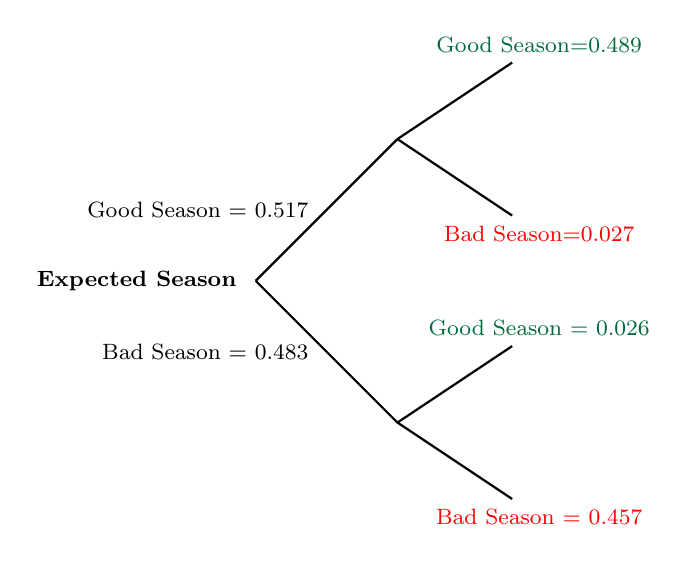
\begin{tikzpicture}[scale=0.6,thick,
    level/.style={level distance=3cm},
    level 2/.style={sibling distance=6cm},
    level 3/.style={sibling distance=4cm}
]
\coordinate
child[grow=right, level distance=0pt] {
        child  {
            child {
                node {{\footnotesize \textcolor{red}{Bad Season = 0.457}}}
                edge from parent 
            }
            child {
                node {{\footnotesize \textcolor{cadmiumgreen}{Good Season = 0.026}}}
                edge from parent
            }
            edge from parent
            node [left] {{\footnotesize Bad Season = 0.483 \ }}
        }
        child {
            child {
                node {{\footnotesize \textcolor{red}{Bad Season=0.027}}}
                edge from parent
            }
            child {
                node {{\footnotesize \textcolor{cadmiumgreen}{Good Season=0.489}}}
                edge from parent  
            }
            edge from parent 
            node [left] {{\footnotesize Good Season = 0.517 \ }}
        }
        node [left] {{\footnotesize \textbf{Expected Season\ \ }}}
    };
\end{tikzpicture}
\end{figure}
\end{frame}

\begin{frame}
\frametitle{Conception and Births: OLD}
\begin{figure}
\hspace{6.0cm}{\footnotesize \textbf{Realized Season}} \vspace{4mm}\\
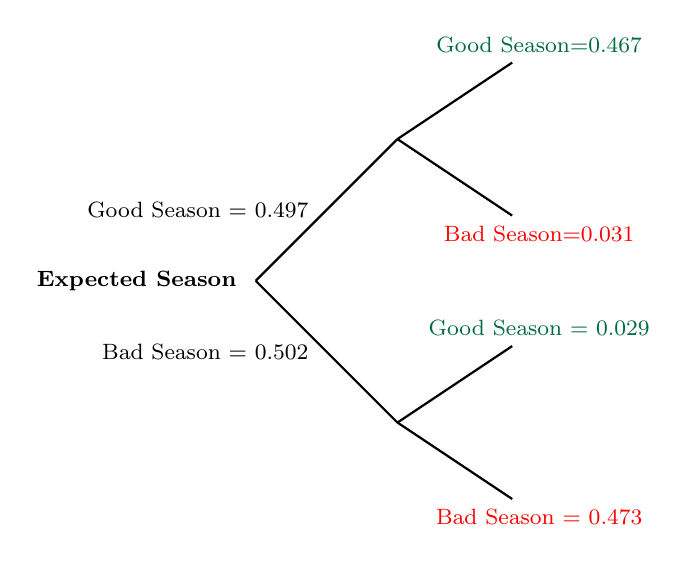
\begin{tikzpicture}[scale=0.6,thick,
    level/.style={level distance=3cm},
    level 2/.style={sibling distance=6cm},
    level 3/.style={sibling distance=4cm}
]
\coordinate
child[grow=right, level distance=0pt] {
        child  {
            child {
                node {{\footnotesize \textcolor{red}{Bad Season = 0.473}}}
                edge from parent 
            }
            child {
                node {{\footnotesize \textcolor{cadmiumgreen}{Good Season = 0.029}}}
                edge from parent
            }
            edge from parent
            node [left] {{\footnotesize Bad Season = 0.502 \ }}
        }
        child {
            child {
                node {{\footnotesize \textcolor{red}{Bad Season=0.031}}}
                edge from parent
            }
            child {
                node {{\footnotesize \textcolor{cadmiumgreen}{Good Season=0.467}}}
                edge from parent  
            }
            edge from parent 
            node [left] {{\footnotesize Good Season = 0.497 \ }}
        }
        node [left] {{\footnotesize \textbf{Expected Season\ \ }}}
    };
\end{tikzpicture}
\end{figure}
\end{frame}

\begin{frame}[label=NVSSQuality]
\frametitle{Birth Quality}
\begin{table}[htbp]\centering
\def\sym#1{\ifmmode^{#1}\else\(^{#1}\)\fi}
\caption{Birth Quality by Age and Season (NVSS 2005-2013)}
\scalebox{0.68}{
\begin{tabular}{l*{7}{c}}
\toprule
                    &\multicolumn{1}{c}{(1)}   &\multicolumn{1}{c}{(2)}   &\multicolumn{1}{c}{(3)}   &\multicolumn{1}{c}{(4)}   &\multicolumn{1}{c}{(5)}   &\multicolumn{1}{c}{(6)}   &\multicolumn{1}{c}{(7)}   \\
                    &       APGAR   & Birthweight   &   Gestation   &         LBW   &   Premature   &        Twin   &        VLBW   \\
\midrule
Aged 25-39          &       0.043***&     130.718***&       0.598***&      -0.055***&      -0.064***&      -0.054***&      -0.010***\\
                    &     [0.004]   &     [2.581]   &     [0.011]   &     [0.001]   &     [0.001]   &     [0.001]   &     [0.000]   \\
Bad Season          &       0.002   &      -5.653   &      -0.011   &       0.004** &       0.002   &       0.001   &      -0.001*  \\
                    &     [0.005]   &     [3.585]   &     [0.015]   &     [0.002]   &     [0.002]   &     [0.001]   &     [0.001]   \\
Young$\times$ Bad S &      -0.005   &      -4.781   &      -0.014   &      -0.001   &       0.001   &       0.001   &       0.002***\\
                    &     [0.005]   &     [3.638]   &     [0.015]   &     [0.002]   &     [0.002]   &     [0.001]   &     [0.001]   \\
College Educ        &       0.045***&      77.112***&       0.181***&      -0.025***&      -0.021***&       0.010***&      -0.006***\\
                    &     [0.001]   &     [0.917]   &     [0.004]   &     [0.000]   &     [0.000]   &     [0.000]   &     [0.000]   \\
&&&&&&&\\
Constant            &       8.756***&    3121.397***&      38.034***&       0.150***&       0.194***&       1.075***&       0.028***\\
                    &     [0.004]   &     [2.775]   &     [0.012]   &     [0.001]   &     [0.001]   &     [0.001]   &     [0.001]   \\
\midrule
R-squared           &        0.00   &        0.00   &        0.00   &        0.00   &        0.00   &        0.00   &        0.00   \\
Observations        &     3551931   &     3603294   &     3610749   &     3613920   &     3613920   &     3613920   &     3613920   \\
\bottomrule
\multicolumn{8}{p{15cm}}{\begin{footnotesize}Sample consists of all
first born children of US-born, white, non-hispanic mothers
\end{footnotesize}}\end{tabular}}\end{table}

\end{frame}

\begin{frame}[label=NVSSQuality]
\frametitle{Birth Quality}
\input{./tables/qualityHeterogeneity.tex}
\end{frame}

\begin{frame}[label=NVSSQualitySeasons]
\frametitle{Birth Quality}
\input{./tables/QualityAllSeasons.tex}
\end{frame}

\begin{frame}[label=sumSpain]
\input{./tables/sumStatsSpain.tex}
\end{frame}

\begin{frame}[label=sumSpainBQ]
\input{./tables/sumSpain.tex}
\end{frame}

\begin{frame}[label=Spainseason]
\frametitle{Season of Birth, Age and Education (Spain)}
\input{./tables/spainBinary.tex}
\end{frame}

\begin{frame}[label=SpainQuality]
\frametitle{Birth Quality (Spain)}
\input{./tables/spainQualityEduc.tex}
\end{frame}


\begin{frame}
\frametitle{Conception and Births: YOUNG (Spain)}
\begin{figure}
\hspace{6.0cm}{\footnotesize \textbf{Realized Season}} \vspace{4mm}\\
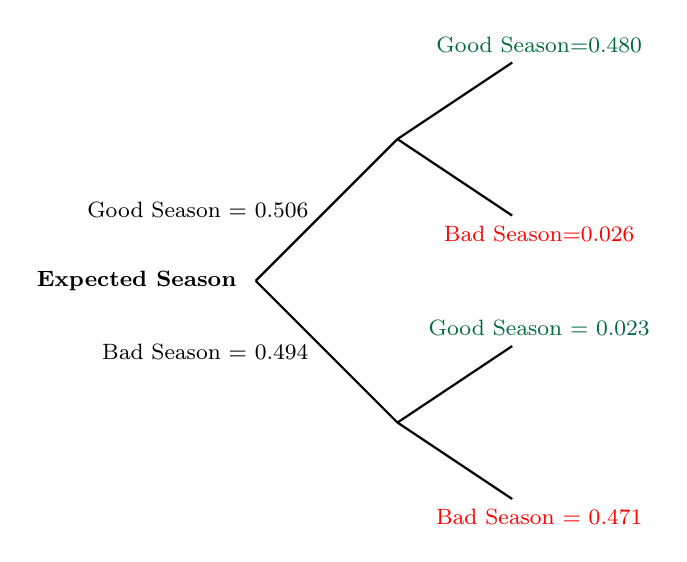
\begin{tikzpicture}[scale=0.6,thick,
    level/.style={level distance=3cm},
    level 2/.style={sibling distance=6cm},
    level 3/.style={sibling distance=4cm}
]
\coordinate
child[grow=right, level distance=0pt] {
        child  {
            child {
                node {{\footnotesize \textcolor{red}{Bad Season = 0.471}}}
                edge from parent 
            }
            child {
                node {{\footnotesize \textcolor{cadmiumgreen}{Good Season = 0.023}}}
                edge from parent
            }
            edge from parent
            node [left] {{\footnotesize Bad Season = 0.494 \ }}
        }
        child {
            child {
                node {{\footnotesize \textcolor{red}{Bad Season=0.026}}}
                edge from parent
            }
            child {
                node {{\footnotesize \textcolor{cadmiumgreen}{Good Season=0.480}}}
                edge from parent  
            }
            edge from parent 
            node [left] {{\footnotesize Good Season = 0.506 \ }}
        }
        node [left] {{\footnotesize \textbf{Expected Season\ \ }}}
    };
\end{tikzpicture}
\end{figure}
\end{frame}

\begin{frame}
\frametitle{Conception and Births: OLD (Spain)}
\begin{figure}
\hspace{6.0cm}{\footnotesize \textbf{Realized Season}} \vspace{4mm}\\
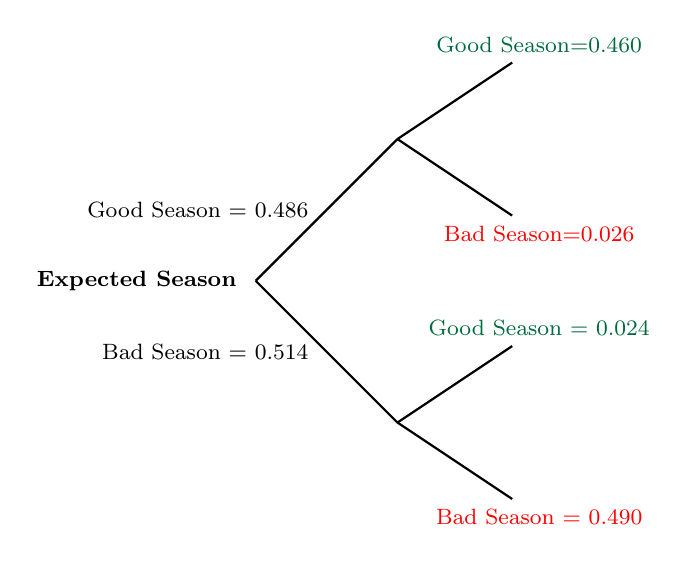
\begin{tikzpicture}[scale=0.6,thick,
    level/.style={level distance=3cm},
    level 2/.style={sibling distance=6cm},
    level 3/.style={sibling distance=4cm}
]
\coordinate
child[grow=right, level distance=0pt] {
        child  {
            child {
                node {{\footnotesize \textcolor{red}{Bad Season = 0.490}}}
                edge from parent 
            }
            child {
                node {{\footnotesize \textcolor{cadmiumgreen}{Good Season = 0.024}}}
                edge from parent
            }
            edge from parent
            node [left] {{\footnotesize Bad Season = 0.514 \ }}
        }
        child {
            child {
                node {{\footnotesize \textcolor{red}{Bad Season=0.026}}}
                edge from parent
            }
            child {
                node {{\footnotesize \textcolor{cadmiumgreen}{Good Season=0.460}}}
                edge from parent  
            }
            edge from parent 
            node [left] {{\footnotesize Good Season = 0.486 \ }}
        }
        node [left] {{\footnotesize \textbf{Expected Season\ \ }}}
    };
\end{tikzpicture}
\end{figure}
\end{frame}


\begin{frame}[label=SpainQuality]
\frametitle{Birth Quality (Spain)}
\input{./tables/spainQualityGestFix.tex}
\end{frame}

\begin{frame}[label=conclusions]
\frametitle{Directions}
\begin{itemize}
\item Estimation of payoffs of season of birth
\item Value of season of birth measured by birth weight, for young and old women
\item Value of SOB and postponing fertility
\item Structural model
\end{itemize}

\end{frame}

\begin{frame}
\begin{center}
{\Large Appendix}
\end{center}
\end{frame}

\begin{frame}[label=model]
\frametitle{Bare-bones model}
%\vspace{10mm}

\begin{itemize}
\item There are two seasons of birth (and two periods):
\begin{itemize}
\item First, Bad Season: $Q4(t-1)\;,\;Q1(t)$
\item Second, Good Season: $Q2(t)\;,\;Q(3)t$
\end{itemize}
\vspace{5mm}
  \begin{picture}(0.0,0.0)
     \put(90,0){\scalebox{0.7}{\includegraphics{./tables/time-line.png}}}
  \end{picture}
\item There are two types of women: \emph{Y}oung (25-39) and \emph{O}ld (40-45)
\item The probability of having a child is higher for young than old women: $p^{Y} > p^{O}$
\item The \emph{biological} (average) quality of the child is higher in the good season than in the bad season: $\mu_{BAD}^{\tau} \leq \mu_{GOOD}^{\tau}$ (e.g., birth weight), where $\tau =\{Y,O\}$.
\item There are \emph{no unwanted pregnancies}
\item Women want to maximize the expected biological quality of their child
\item \emph{Both} types of women are \emph{risk neutral}
\item Each type of woman can play two lotteries: Bad Season or Good Season.
\end{itemize}
\end{frame}

\begin{frame}[label=model]
\frametitle{Bare-bones model}
%\vspace{10mm}

\begin{itemize}
\item If a woman goes for the first season, and she is unsuccessful, she has a second chance in the good season.
\item If a woman goes for the second season, and she is unsuccessful, she has no second chance!
\item The expected payoff for a young woman when going for the \textcolor[rgb]{1.00,0.00,0.00}{bad season} is
    $$\displaystyle \textcolor[rgb]{1.00,0.00,0.00}{p^Y\mu_{BAD}^Y + (1-p^Y)p^Y\mu_{GOOD}^Y}   $$
\item The expected payoff for a young woman when going for the \textcolor[rgb]{0.00,0.07,1.00}{good season} is
    $$\displaystyle \textcolor[rgb]{0.00,0.07,1.00}{p^Y\mu_{GOOD}^Y} $$
\item A young woman goes for the good season if and only if
    $$\displaystyle p^Y\mu_{GOOD}^Y \geq \mu_{BAD}^Y $$
\item By the same token, an old woman goes for the bad season if and only if
    $$\displaystyle p^O\mu_{GOOD}^O \geq \mu_{BAD}^O $$
\end{itemize}
\end{frame}


\begin{frame}
\frametitle{First Birth Rates by Mother's Age: 35-39 vs. 40-44}
\begin{center}
\includegraphics[scale=0.3]{./tables/Figure_1.png}
\end{center}
\end{frame}

\begin{frame}
\frametitle{First Birth for Mother's Age 40-44 by Race and Ethnicity}
\begin{center}
\includegraphics[scale=0.3]{./tables/Figure_3.png}
\end{center}
\end{frame}

\begin{frame}[label=NVSSseason2]
\frametitle{Season of Birth, Age and Education (Birth Order=2)}
\begin{table}[htbp]\centering
\def\sym#1{\ifmmode^{#1}\else\(^{#1}\)\fi}
\caption{Birth Quarter and Age (NVSS 2005-2013)}
\scalebox{0.8}{
\begin{tabular}{l*{4}{c}}
\toprule
                    &\multicolumn{1}{c}{(1)}   &\multicolumn{1}{c}{(2)}   &\multicolumn{1}{c}{(3)}   &\multicolumn{1}{c}{(4)}   \\
                    & Good Season   & Good Season   & Good Season   & Good Season   \\
\midrule
Aged 25-39          &       0.019***&       0.019***&       0.020***&       0.006   \\
                    &     [0.001]   &     [0.001]   &     [0.002]   &     [0.005]   \\
College Educ        &               &               &       0.010***&      -0.005   \\
                    &               &               &     [0.001]   &     [0.005]   \\
College$\times$ Aged 25-39&               &               &               &       0.015***\\
                    &               &               &               &     [0.005]   \\
Constant            &       0.497***&       0.497***&       0.488***&       0.501***\\
                    &     [0.001]   &     [0.001]   &     [0.002]   &     [0.005]   \\
\midrule
R-squared           &        0.00   &        0.00   &        0.00   &        0.00   \\
Observations        &     4871628   &     4871628   &     3613920   &     3613920   \\
Year FE&&Y&Y&Y\\ \bottomrule
\multicolumn{5}{p{12cm}}{\begin{footnotesize}Sample consists of all
first born children of US-born, white, non-hispanic mothers
\end{footnotesize}}\end{tabular}}\end{table}

\end{frame}

\begin{frame}[label=NVSSQuality2]
\frametitle{Birth Quality (Birth Order=2)}
\begin{table}[htbp]\centering
\def\sym#1{\ifmmode^{#1}\else\(^{#1}\)\fi}
\caption{Birth Quality by Age and Season (NVSS 2005-2013)}
\scalebox{0.68}{
\begin{tabular}{l*{7}{c}}
\toprule
                    &\multicolumn{1}{c}{(1)}   &\multicolumn{1}{c}{(2)}   &\multicolumn{1}{c}{(3)}   &\multicolumn{1}{c}{(4)}   &\multicolumn{1}{c}{(5)}   &\multicolumn{1}{c}{(6)}   &\multicolumn{1}{c}{(7)}   \\
                    &       APGAR   & Birthweight   &   Gestation   &         LBW   &   Premature   &        Twin   &        VLBW   \\
\midrule
Aged 25-39          &       0.043***&     130.718***&       0.598***&      -0.055***&      -0.064***&      -0.054***&      -0.010***\\
                    &     [0.004]   &     [2.581]   &     [0.011]   &     [0.001]   &     [0.001]   &     [0.001]   &     [0.000]   \\
Bad Season          &       0.002   &      -5.653   &      -0.011   &       0.004** &       0.002   &       0.001   &      -0.001*  \\
                    &     [0.005]   &     [3.585]   &     [0.015]   &     [0.002]   &     [0.002]   &     [0.001]   &     [0.001]   \\
Young$\times$ Bad S &      -0.005   &      -4.781   &      -0.014   &      -0.001   &       0.001   &       0.001   &       0.002***\\
                    &     [0.005]   &     [3.638]   &     [0.015]   &     [0.002]   &     [0.002]   &     [0.001]   &     [0.001]   \\
College Educ        &       0.045***&      77.112***&       0.181***&      -0.025***&      -0.021***&       0.010***&      -0.006***\\
                    &     [0.001]   &     [0.917]   &     [0.004]   &     [0.000]   &     [0.000]   &     [0.000]   &     [0.000]   \\
&&&&&&&\\
Constant            &       8.756***&    3121.397***&      38.034***&       0.150***&       0.194***&       1.075***&       0.028***\\
                    &     [0.004]   &     [2.775]   &     [0.012]   &     [0.001]   &     [0.001]   &     [0.001]   &     [0.001]   \\
\midrule
R-squared           &        0.00   &        0.00   &        0.00   &        0.00   &        0.00   &        0.00   &        0.00   \\
Observations        &     3551931   &     3603294   &     3610749   &     3613920   &     3613920   &     3613920   &     3613920   \\
\bottomrule
\multicolumn{8}{p{15cm}}{\begin{footnotesize}Sample consists of all
first born children of US-born, white, non-hispanic mothers
\end{footnotesize}}\end{tabular}}\end{table}

\end{frame}


\begin{frame}[label=NVSStwin]
\frametitle{Season of Birth, Age and Education (Twins)}
\input{./tables/NVSSBinaryTwin.tex}
\end{frame}

\begin{frame}[label=NVSSQualitytwin]
\frametitle{Birth Quality (Twins)}
\input{./tables/NVSSQualityTwin.tex}
\end{frame}

\begin{frame}[label=NVSSFD]
\frametitle{Season of Birth, Age and Education (Fetal Deaths)}
\input{./tables/NVSSBinaryFDeathsOnly.tex}
\end{frame}




\end{document}
%********************************************************************************



